% Make nice A4 pages for print:
%\usepackage{pgfpages}
%\pgfpagesuselayout{resize to}[a4paper,border shrink=5mm,landscape]

\beamertemplatenavigationsymbolsempty

\setbeamertemplate{bibliography item}[text]

\usepackage[type={CC},modifier={by-sa},version={4.0}]{doclicense}

\usepackage[utf8]{inputenc}
\usepackage{hyperref}
\usepackage{breakurl}
\usepackage{graphicx}
\usepackage{pgfplots}
\usepackage{pgf}
\usepackage{tikz}
\usetikzlibrary{positioning}
\usetikzlibrary{arrows}
\usetikzlibrary{decorations.markings}
\usetikzlibrary{calc}
\usetikzlibrary{matrix}
\usetikzlibrary{shapes}
\usetikzlibrary{decorations.pathmorphing}
\usetikzlibrary{fit}
\usetikzlibrary{backgrounds}
\usetikzlibrary{plotmarks}
\usepackage{stmaryrd}
\usepackage{listings}
\usepackage{pdflscape}
\usepackage{perpage}
\usepackage{appendixnumberbeamer}

%\usepackage[thmmarks,amsmath,amsthm]{ntheorem} % already included in beamer
\usepackage{thm-restate}

\usepackage[sort&compress,numbers]{natbib}  % to be have \citet, \citeauthor, \citeyear

\MakePerPage{footnote}

\tikzstyle{o}=[r,ppBlue]
\tikzstyle{r}=[thick,rectangle,align=center]
\tikzstyle{t}=[r,ppTrans] %,font=\bfseries]
\tikzstyle{dd}=[densely dashed]
\tikzstyle{n}=[r,ppBlue]
\tikzstyle{p}=[r,ppRed]
\tikzstyle{ppRed}  =[draw=red,  fill=  red!20]
\tikzstyle{ppBlue} =[draw=blue, fill= blue!20]
\tikzstyle{ppGreen}=[draw=green,fill=green!20]
\tikzstyle{ppTrans}=[draw=none, fill=none]

\usetheme{Warsaw}

\useoutertheme[subsection=true]{smoothbars}
%\useoutertheme[subsection=false]{miniframes}

\definecolor{bblue}{HTML}{D7DF01}	% yellow-ish actually, for better black/white printing
\definecolor{rred}{HTML}{C0504D}
\definecolor{ggreen}{HTML}{9BBB59}
\definecolor{ppurple}{HTML}{9F4C7C}
\definecolor{lightgray}{rgb}{0.3,0.3,0.3}
\definecolor{lightergray}{rgb}{0.9,0.9,0.9}
\definecolor{UniBlue}{RGB}{83,121,170}

\DeclareTextFontCommand\textintro{\normalfont\bfseries\itshape} % nice!
\newcommand{\intro}[2][]
{%
	\textintro{#2}%
}
\newcommand{\empha}[2][]
{%
	\emph{#2}%
}

%\theoremstyle{plain}
\newcounter{reqcounter}
\newtheorem{requirement}[reqcounter]{Requirement}

%setbeamercolor{structure}{fg=violet}

\makeatletter
\def\th@task{%
    \normalfont % body font
    \setbeamercolor{block title example}{bg=orange,fg=white}
    \setbeamercolor{block body example}{bg=orange!20,fg=black}
    \def\inserttheoremblockenv{exampleblock}
  }
\makeatother

\theoremstyle{task}
\newtheorem{task}{Task}

\newenvironment{assignment}%
{%\setbeamercolor{background canvas}{bg=violet}%
%\setbeamercolor{structure}{fg=cyan!90!black}%
 \setbeamercolor{frametitle}{bg=orange,fg=white}
\begin{frame}}%
{\end{frame}}%

\AtBeginSection[]{
  \begin{frame}
  \vfill
  \centering
  \begin{beamercolorbox}[sep=8pt,center,shadow=true,rounded=true]{title}
    \usebeamerfont{title}\insertsectionhead\par%
  \end{beamercolorbox}
  \tableofcontents
  \vfill
  \end{frame}
}




\pgfplotsset{compat=1.14}
\author{Markus Raab}


\title{L07 Strategies for Reduction of Misconfiguration}
\date{05.05.2021}

\begin{document}


%%%%%%%%%%%%%%%%%%%%%%%%%%%%%%%%%%%%%%%%%% 
\section{Terms and Properties}

\begin{frame}
	\frametitle{Learning Outcomes}
	Students will be able to
	\begin{itemize}
	\item remember terms of properties of CM.
	\item remember various strategies for reduction of misconfiguration.
	\item find unused settings.
	\end{itemize}
\end{frame}

\begin{frame}<2>[label=iac]
	\frametitle{Infrastructure as Code}

	\only<2>{
	Configuration settings are an instantiation of the configuration specifications.
	\vspace{1em}

	The instantiation code is implemented by \textbf{CM code}.
	\vspace{1em}

	\textbf{Auditability:}
	Being informed about status and changes in the infrastructure.
	\vspace{1em}

	\begin{alertblock}{Goal}
	Single Source of Truth
	\end{alertblock}
	}
\end{frame}

\begin{frame}
	\frametitle{Configuration Drift}

	is a derivation of the ``Single Source of Truth'' (the CM code).

	\vspace{1em}
	It is caused by:

	\pause

	\begin{itemize}[<+-| alert@+>]
	\item manual configuration changes by administrators
	\item manual configuration changes by end users
	\item differences in updates (e.g., skipped or failed updates)
	\item failed attempts to change configuration
	\item applying different versions of CM code
	\item non-idempotent CM Code
	\item \dots
	\end{itemize}
\end{frame}

\begin{frame}<1>[label=idempotence]
	\frametitle{Idempotence}

	\only<1>{
	idem + potence (same + power)
	\vspace{2em}
	}

	\only<1,3>{
	Yield same result with any number of applications ($n\ge1$):
		
	\[
		f(f(x))=f(x)
	\]
	}
\end{frame}

\begin{frame}
	\frametitle{Example}
	\citet{waldemar2013testing} tested 298 Chef scripts, of which 92 were non-idempotent:

	\begin{itemize}[<+-| alert@+>]
	\item \texttt{/etc/timezone} rewritten by package tzdata
	\item tomcat6: files copied by user if \texttt{/etc/tomcat6/tomcat6.conf} does not exist but copy fails because later step creates \texttt{/etc/tomcat6/logging.properties} as root.
	\item mongodb: if installation fails, the group ``mongodb'' does not exist, failing at later tasks creating directories using this group
	\end{itemize}
\end{frame}

\begin{frame}
	\citet{wadler2003xml} describe two further properties:
	\vspace{2em}

	\begin{description}
	\item[Self-describing]
	means that from the configuration file alone we are able to derive the correct data structure~\cite{wadler2003xml}.

	\item[Round-tripping]
	means that if a data structure is serialized and then parsed again, we end up with an identical data structure~\cite{wadler2003xml}.
	\end{description}

	The data structure could be a KeySet.

	\pause

	\vspace{2em}
	Round-tripping is a prerequisite of idempotence.
\end{frame}


\begin{frame}[fragile]
	\frametitle{Examples}

	XML has neither of the last two properties~\citet{wadler2003xml}:

	\begin{itemize} %[<+-| alert@+>]
	\item internal representation crucially depends on XML schema
	\item union of integer and strings
	\begin{code}[gobble=4]
	intOrStr { "one", "2", 3 }
	<fact>one 2 3</fact>
	intOrStr { "one",  2,  3 }
	\end{code}

	\end{itemize}
\end{frame}



%%%%%%%%%%%%%%%%%%%%%%%%%%%%%%%%%%%%%%%%%% 
\section{Pitfalls}

\begin{frame}[fragile]
	\frametitle{Harmful Defaults~\cite{xu2015hey}}
	\begin{itemize}
	\item Problem: Two major data losses on a dozen machines.
	\item Cause:
	Stayed with the default values of the data-path settings
	(e.g., ^dfs.name.dir^, ^dfs.data.dir^) which point to locations in ^/tmp^.
	Thus, after the machines reboot, data losses occur.
	``One of the common problems from users.'' (from Cloudera)
	\item up to \p{53} of misconfigurations is due to staying at defaults
	\item \p{17} to \p{48} of configuration issues are about difficulties in finding settings
	\end{itemize}
\end{frame}

\begin{frame}
	\begin{alertblock}{Question}
	What do we want to test?
	\end{alertblock}

	\pause
	\begin{itemize}
	\item That settings do what they should (devs and admins)
	\item That settings are properly validated (devs~\cite{xu2013blame})
	\item Regression tests~\cite{qu2008configuration}
	\pause
	\vspace{1em}
	\item Are all settings implemented?
	\item Are all settings used in tests?
	\item Are there unused settings in the code?
	\end{itemize}
\end{frame}

\begin{frame}
	Matt Welsh from Google wrote in 2013:\footnote{What I wish systems researchers would work on. Retrieved from http://matt-welsh.blogspot.com/2013/05/what-i-wish-systems-researchers-would.html.}

	\vspace{2em}

	\emph{``Of course we have extensive testing infrastructure, but the ‘hard’ problems always
	come up when running in a real production environment, with real traffic and real
	resource constraints. Even integration tests and canarying are a joke compared to
	how complex production-scale systems are.''}
\end{frame}

\lstDeleteShortInline^
\begin{frame}
	\frametitle{\citet{jin2014configurations}}

	\begin{itemize}
	\item Wants to improve configuration-aware testing and debugging
	\item Manual investigations for three applications
	\item Finds 1957 settings in Firefox ($2^{846} * 3^{1111}$) and \\
		36322 in LibreOffice ($2^{4433} * 3^{31889}$)
	\item Finds unused settings: settings only in the source code
	\item Finds configuration settings which are not specified
	\end{itemize}

	\begin{requirement}
	Configuration setting traceability is a necessity.
	\end{requirement}

	\begin{alertblock}{Idea}
	Code generation helps to trace settings and to find unused settings.
	\end{alertblock}
\end{frame}
\lstMakeShortInline[postbreak=,keywordstyle={},showspaces=no]^
%XXX

%Other requirements they have:
%\begin{frame}
%	\frametitle{Requirements \cite{jin2014configurations}}
%	\begin{requirement}
%	Configuration Modeling Should Merge Multiple Layers.
%	\end{requirement}
%	\begin{requirement}
%	Analysis Tools Need to Cross the Programming Language Barrier
%	\end{requirement}
%	\begin{requirement}
%	Configuration State Capture or Approximation Techniques are Needed
%	\end{requirement}
%\end{frame}

\begin{frame}
	\frametitle{Testing by developers:}
	\begin{itemize}[<+-| alert@+>]
	\item ConfErr~\cite{keller2008conferr} uses models of key board layout, psychology and linguistics.
	Tool injects possible misconfiguration.
	\item Spex~\cite{xu2013blame} analyzes the source code to find misconfigurations.
	As by-product it extracts internal specifications (including transformation bugs).
	\item External specification can be directly used to generate test cases.
	\item Find unused configuration settings.
	\end{itemize}
\end{frame}

%%%%%%%%%%%%%%%%%%%%%%%%%%%%%%%%%%%%%%%%%% 
\section{Unused Settings}

\begin{frame}
	\frametitle{Trend Configuration Files (Recapitulation)}
	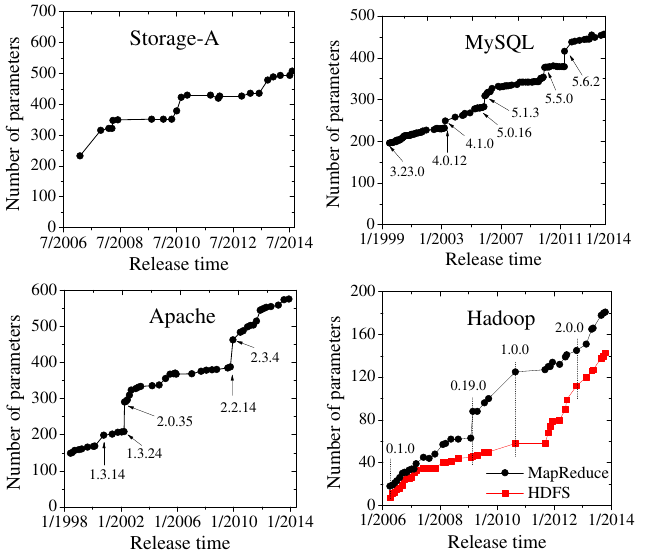
\includegraphics[scale=0.5]{pics/trend.png}
	\citet{xu2015hey}
\end{frame}

\begin{frame}[fragile]
	\frametitle{Unnecessary Settings~\cite{xu2015hey}}
	\begin{itemize}
	\item Configuration Parameter: ^dfs.namenode.tolerate.heartbeat.multiplier^
	\item Developers' Discussion:
	Since we are not sure what is a good choice, how about making it
	configurable?
	We should add a configuration option for it. Even if it's unlikely to
	change, if someone does want to change it they'll thank us that they
	don't have to change the code/recompile to do so.
	\item Real-World Usage:
	\begin{itemize}
	\item No usage found by searching the entire mailing lists and Google.
	\item No usage reported in a survey of 15 Hadoop users in UCSD.
	\end{itemize}
	\end{itemize}
\end{frame}

\begin{frame}
	\frametitle{Unnecessary Settings~\cite{xu2015hey}}
	\begin{itemize}
	\item \p{6} to \p{17} of settings set by majority
	\item up to \p{54} are seldom set
	\item up to \p{47} of numeric settings have no more than five distinct values
	\end{itemize}
\end{frame}

\begin{frame}
	\frametitle{Reduction}
	\methodQuestion{}
	\question{Why do you think configuration should be reduced?}
	\begin{itemize}
	\item to simplify code maintenance (\p{50}),
	\item to prevent errors and misconfiguration (\p{43}),
	\item to provide better user experience (\p{40}),
	\item \textbf{\question{I do not think it should be reduced} (\p{30})},
	\item because they prefer auto-detection (\p{29}) \\ (with a possibility to override configuration settings: \p{32}),
	\item \question{because use-cases which are rarely used should not be supported} (\p{13}),
	\item \question{never find time for this task} (\p{9}), and
	\item \question{because only standard use-cases should be supported} (\p{1})
	\end{itemize}
\end{frame}

\begin{frame}
	\frametitle{Limitations of Zero-Configuration}
	\begin{itemize}
	\item e.g. gpsd\footnote{\url{www.aosabook.org/en/gpsd.html}}
	\pause
	\item broken hardware or protocols
	\item auto-detection may go wrong
	\item the configuration actually lives elsewhere \\ (e.g., in the GPS devices)
	\end{itemize}
\end{frame}

\begin{frame}
	\frametitle{Visibility}
	\begin{itemize}
	\item idea: show only relevant settings for specific user group
	\item or disallow editing: accessibility
	\pause
	\item requires user-feedback loops~\cite{xu2015hey}
	\item most-used settings should be best visible (or even enforce them to be changed: against harmful defaults)
	\item think of your users (administrators), \\ only expose what users need
	\item write an rationale why someone needs it
	\pause
	\item visibility should not be an excuse to add not-needed settings
	\end{itemize}
\end{frame}

\begin{frame}[fragile]
	\frametitle{Example}
	\begin{code}[gobble=4]
	[slapd/threads/listener]
	visibility:=developer

	[slapd/access/#]
	visibility:=user
	\end{code}
\end{frame}


\begin{frame}
	\frametitle{Find Unused Settings}

	%contextual value not yet introduced:
	%\ExecuteMetaData[../book/implications.tex]{algorithm-first}
	The first (optional) step of the algorithm is:
	\begin{itemize}
	\item Run all tests with code coverage.
	\item Check if generated code is executed.
	\item If it is, we know that the configuration setting is used in a test case.
	Otherwise, we know it is not tested by the test suite.
	All these untested configuration settings are remembered as candidates for the second step.
	\end{itemize}
\end{frame}

\begin{frame}[fragile]
	\small
	\fontsize{10}{0}\selectfont
	\begin{code}[gobble=4,language=Cpp]
	KeySet findUnusedSettings (KeySet untestedSettings,
				   KDB kdb,
				   Builder build)
	{
	   KeySet unusedSettings = {};
	   KeySet configurationSpecification;
	   kdb.get (configurationSpecification);

	   for (candidate: untestedSettings)
	   {
	       configurationSpecification.remove (candidate);
	       kdb.set (configurationSpecification);
	       build.recompile ();
	       if (build.wasSuccessful ())
	       {
	          unusedSettings.append (candidate);
	       }
	       configurationSpecification.append (candidate);
	   }

	   kdb.set (configurationSpecification);
	   return unusedSettings;
	}
	\end{code}
\end{frame}

\begin{frame}
	\frametitle{Conclusion}

	\begin{itemize}[<+-| alert@+>]
	\item Definition and challenges in configuration management.
	\item Properties: self-describing, idempotent, round-tripping.
	\item Awareness and responsibility needed.
	\item Avoidance of misconfiguration is combined effort of devs and admins.
	\end{itemize}
\end{frame}


%%%%%%%%%%%%%%%%%%%%%%%%%%%%%%%%%%%%%%%%%%
\section{Meeting}

\subsection{Recapitulation}

\againframe<1,2>{iac}

%TODO: deduplicate
\begin{frame}
	\frametitle{Configuration Drift}

	\pause

	is a derivation of the ``Single Source of Truth'' (the CM code).

	\vspace{1em}
	It is caused by:

	\begin{itemize} %[<+-| alert@+>]
	\item manual configuration changes by administrators
	\item manual configuration changes by end users
	\item differences in updates (e.g., skipped or failed updates)
	\item failed attempts to change configuration
	\item applying different versions of CM code
	\item non-idempotent CM Code
	\item \dots
	\end{itemize}
\end{frame}

%\againframe<2,3>{idempotence}

\begin{frame}
	\frametitle{Properties (Recapitulation)}

	\begin{task}
	What is idempotent, self-describing, round-tripping configuration?
	\end{task}

	\pause


	\begin{description}
	\item[Idempotent]
	yield the same configuration with any number of applications from CM code ($n\ge1$)~\cite{waldemar2013testing}:
	\[
		f(f(x))=f(x)
	\]
	needed to guarantee repeatability

	\item[Self-describing]
	means that from the configuration file alone we are able to derive the correct data structure~\cite{wadler2003xml}.

	\item[Round-tripping]
	means that if a data structure is serialized and then parsed again, we end up with an identical data structure~\cite{wadler2003xml}.
	\end{description}

	The data structure could be a KeySet.
\end{frame}

\begin{frame}
	\frametitle{Pitfalls of CM}

	\pause

	\begin{itemize}
	\item too many (unused) settings
	\item no external specification
	\item too complicated configuration design
	\item harmful defaults
	\item no configuration-aware tests
	\item settings and specs not synchronized
	\end{itemize}
\end{frame}

\begin{frame}
	\frametitle{Reduction of Configuration Settings}

	\pause

	\begin{itemize}
	\item Zero-Configuration (auto detection)
	\item Visiblity
	\item Find unused settings (code generator needed)
	\end{itemize}
\end{frame}


\subsection{Assignments}

\begin{assignment}
	Slides for talk in TUWEL \textbf{and} private git repo:

	\begin{itemize}
	\item 12 May: submission
	\item 26 May: peer review
	\end{itemize}
\end{assignment}

\begin{assignment}
	Today: Correction H2

	Upcoming: H3, T3
\end{assignment}


\subsection{TW}

\begin{frame}
	\frametitle{Today}

	\begin{enumerate}
	\item Give yourselves roles (admin, dev, user)
	\item Split the goals and tasks among them.
	\end{enumerate}
\end{frame}

\begin{frame}
	\frametitle{Preparation}

	\begin{enumerate}
	\item Do homework as described in L08 materials.
	\end{enumerate}
\end{frame}

\begin{frame}
	\frametitle{Outlook}

	In the next lecture (LTW):

	\begin{enumerate}
	\item Create together an architecture that fulfils the goals.
	\item Present that architecture, explain the concepts, show which technologies you found.
	\end{enumerate}
\end{frame}



\appendix

\begin{frame}[allowframebreaks]
	\bibliographystyle{plainnat}
	\bibliography{../shared/elektra.bib}
\end{frame}



\end{document}
